%% bare_conf_compsoc.tex
%% V1.4b
%% 2015/08/26
%% by Michael Shell

\documentclass[conference,compsoc]{IEEEtran}

% *** MISC UTILITY PACKAGES ***
%
\usepackage{ifpdf}
% Heiko Oberdiek's ifpdf.sty is very useful if you need conditional
% compilation based on whether the output is pdf or dvi.
% usage:
% \ifpdf
%   % pdf code
% \else
%   % dvi code
% \fi
\usepackage{verbatim}
% *** CITATION PACKAGES ***
%
\ifCLASSOPTIONcompsoc
  % IEEE Computer Society needs nocompress option
  % requires cite.sty v4.0 or later (November 2003)
  \usepackage[nocompress]{cite}
\else
  % normal IEEE
  \usepackage{cite}
\fi

% *** GRAPHICS RELATED PACKAGES ***
%
\ifCLASSINFOpdf
  % \usepackage[pdftex]{graphicx}
  % declare the path(s) where your graphic files are
  % \graphicspath{{../pdf/}{../jpeg/}}
  % and their extensions so you won't have to specify these with
  % every instance of \includegraphics
  % \DeclareGraphicsExtensions{.pdf,.jpeg,.png}
\else
  % or other class option (dvipsone, dvipdf, if not using dvips). graphicx
  % will default to the driver specified in the system graphics.cfg if no
  % driver is specified.
  % \usepackage[dvips]{graphicx}
  % declare the path(s) where your graphic files are
  % \graphicspath{{../eps/}}
  % and their extensions so you won't have to specify these with
  % every instance of \includegraphics
  % \DeclareGraphicsExtensions{.eps}
\fi


% *** MATH PACKAGES ***
%
\usepackage{amsmath}


% IEEEtran contains the IEEEeqnarray family of commands that can be used to
% generate multiline equations as well as matrices, tables, etc., of high
% quality.


% *** SUBFIGURE PACKAGES ***
%\ifCLASSOPTIONcompsoc
%  \usepackage[caption=false,font=footnotesize,labelfont=sf,textfont=sf]{subfig}
%\else
%  \usepackage[caption=false,font=footnotesize]{subfig}
%\fi

% *** FLOAT PACKAGES ***
%
%\usepackage{fixltx2e}
% fixltx2e, the successor to the earlier fix2col.sty, was written by
% Frank Mittelbach and David Carlisle. This package corrects a few problems
% in the LaTeX2e kernel, the most notable of which is that in current
% LaTeX2e releases, the ordering of single and double column floats is not
% guaranteed to be preserved. Thus, an unpatched LaTeX2e can allow a
% single column figure to be placed prior to an earlier double column
% figure.
% Be aware that LaTeX2e kernels dated 2015 and later have fixltx2e.sty's
% corrections already built into the system in which case a warning will
% be issued if an attempt is made to load fixltx2e.sty as it is no longer
% needed.
% The latest version and documentation can be found at:
% http://www.ctan.org/pkg/fixltx2e


%\usepackage{stfloats}
% stfloats.sty was written by Sigitas Tolusis. This package gives LaTeX2e
% the ability to do double column floats at the bottom of the page as well
% as the top. (e.g., "\begin{figure*}[!b]" is not normally possible in
% LaTeX2e). It also provides a command:
%\fnbelowfloat
% to enable the placement of footnotes below bottom floats (the standard
% LaTeX2e kernel puts them above bottom floats). This is an invasive package
% which rewrites many portions of the LaTeX2e float routines. It may not work
% with other packages that modify the LaTeX2e float routines. The latest
% version and documentation can be obtained at:
% http://www.ctan.org/pkg/stfloats
% Do not use the stfloats baselinefloat ability as the IEEE does not allow
% \baselineskip to stretch. Authors submitting work to the IEEE should note
% that the IEEE rarely uses double column equations and that authors should try
% to avoid such use. Do not be tempted to use the cuted.sty or midfloat.sty
% packages (also by Sigitas Tolusis) as the IEEE does not format its papers in
% such ways.
% Do not attempt to use stfloats with fixltx2e as they are incompatible.
% Instead, use Morten Hogholm'a dblfloatfix which combines the features
% of both fixltx2e and stfloats:
%
% \usepackage{dblfloatfix}
% The latest version can be found at:
% http://www.ctan.org/pkg/dblfloatfix


% *** PDF, URL AND HYPERLINK PACKAGES ***
%
%\usepackage{url}
% url.sty was written by Donald Arseneau. It provides better support for
% handling and breaking URLs. url.sty is already installed on most LaTeX
% systems. The latest version and documentation can be obtained at:
% http://www.ctan.org/pkg/url
% Basically, \url{my_url_here}.

% correct bad hyphenation here
\hyphenation{op-tical net-works semi-conduc-tor}


\begin{document}
%
% paper title
\title{A Salient Region Detector for Structured Images}


% author names and affiliations
% use a multiple column layout for up to three different
% affiliations
\author{\IEEEauthorblockN{Elena Ranguelova}
\IEEEauthorblockA{Netherlands eScience Center\\
Amsterdam, The Netherlands\\
Email: E.Ranguelova@esciencecenter.nl}
}

% make the title area
\maketitle

% As a general rule, do not put math, special symbols or citations
% in the abstract
\begin{abstract}
% background
Finding correspondences between two images of the same scene or object, taken from different viewpoints and conditions, is a challenging task. Analyzing scientific imagery often requires the detected local features to match meaningful image structures, thus adding more complexity to the task. Ecologists use photo-identification methods in their population studies and conservational efforts. In addition to the task of identifying an individual plant or animal or classifying species, precise phenotypic measurements are often  needed.
% objectives
Generic detectors, such as the renowned Maximally Stable Extremal Regions (MSER) perform very well on structured images, but have difficulties with blur, lighting and increased resolution. The detected regional features do not always correspond to semantically meaningful structures and their large number hampers scalability. 
%methods
This paper proposes a Data-driven Morphology Salient Regions (DMSR) detector which overcomes the above limitations. A new binarization algorithm uses a threshold derived from the data. The binary image is analyzed for saliency using morphology. 
% results & conclusions
DMSR shows transformation invariance and comparable repeatability to MSER on three evaluation benchmarks while having better invariance to lighting, blur and increased image resolution. This is achieved via significantly fewer detected regions, leading to better scalability. Some preliminary results on animal and plant images, indicate that DMSR could be a suitable approach for such application as the detected regions match semantically interesting structures well. The paper also introduces OxFrei - a dataset for transformation-independent detection evaluation. All experimental results, well-documented dataset and the open-source software are available online making the research reported in this paper repeatable.

\end{abstract}

% no keywords




% For peer review papers, you can put extra information on the cover
% page as needed:
% \ifCLASSOPTIONpeerreview
% \begin{center} \bfseries EDICS Category: 3-BBND \end{center}
% \fi
%
% For peerreview papers, this IEEEtran command inserts a page break and
% creates the second title. It will be ignored for other modes.
\IEEEpeerreviewmaketitle


\section{Introduction}
% no \IEEEPARstart
\label{sec:intro}
The first fundamental step in numerous computer vision applications (wide baseline stereo matching, image retrieval, visual mining, etc.\,) is to reliably and repeatedly find  the correspondence between a pair of different images of the same scene \cite{Matas2002BMVC, Rodriguez2013, EscaleraCVPR07}. One class of methods- {\em region detectors} find distinct (salient) regions, which correspond to the same image patches, detected independently in each image. The detectors must be {\em covariant} (often called {\em invariant}) to, usually, {\em affine} transformations and various photometric distortions. 

A decade ago, a performance evaluation paper by the Visual Geometry Group in Oxford compared existing region detectors \cite{Mikolajczyk:2005}. 
A clear conclusion of the comparison was that {\em  Maximally Stable Extremal Regions (MSER)} is the best performing detector for {\em structured} scenes, e.g., those containing homogeneous regions with distinctive boundaries \cite{Matas2002BMVC}. MSER has become the de-facto standard in the field, e.g., it is in the MATLAB Computer Vision Systems Toolbox and OpenCV. Despite its success, the detector has several drawbacks: it is sensitive to image blur; it produces nested and redundant regions and its performance degrades with the increase of image resolution \cite{CorRos2013}. Analysis in geometric scale-space have showed that the formulation of the region stability criterion makes MSER prefer regular shapes \cite{Kimmel11}.

\begin{comment}
\begin{figure}[htb]

\begin{minipage}[b]{.48\linewidth}
  \centering
  \centerline{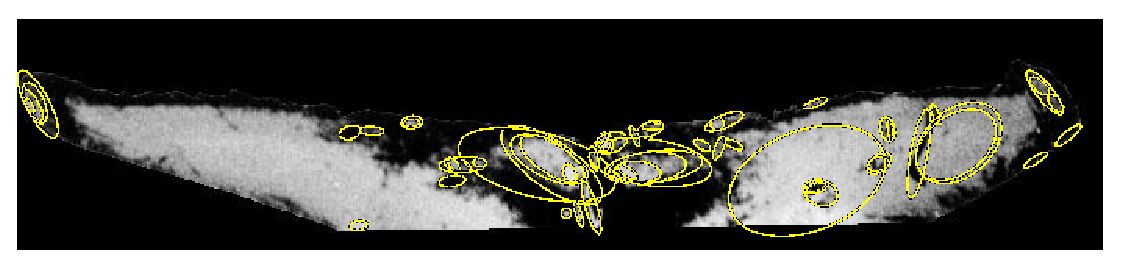
\includegraphics[width=4cm]{./Figs/mserTailA}}
\end{minipage}
\begin{minipage}[b]{0.51\linewidth}
  \centering
  \centerline{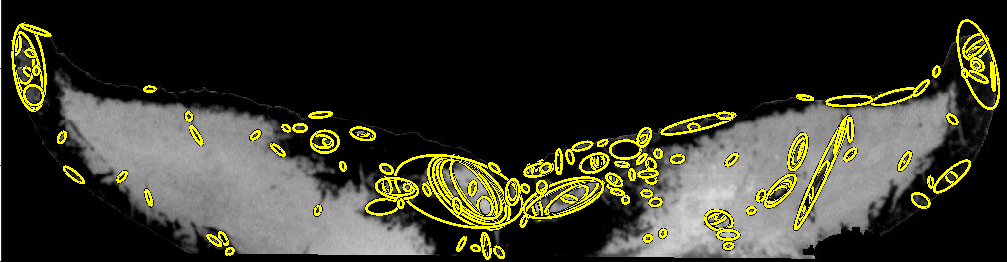
\includegraphics[width=4cm]{./Figs/mserTailB}}
\end{minipage}
\hfill
\begin{minipage}[b]{.48\linewidth}
  \centering
  \centerline{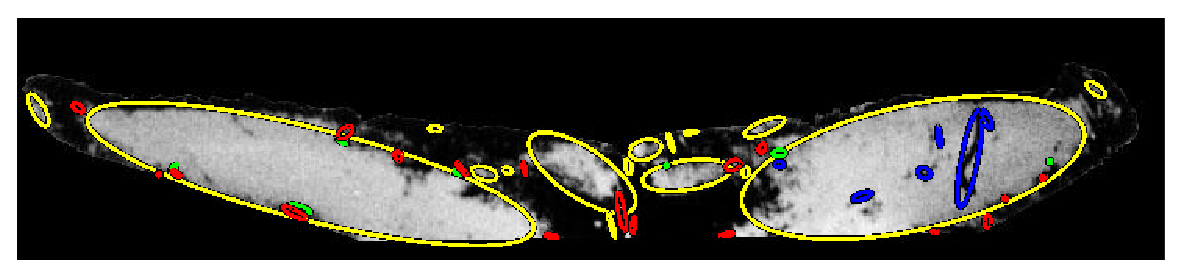
\includegraphics[width=4cm]{./Figs/dmsrTailA}}
\end{minipage}
\begin{minipage}[b]{0.51\linewidth}
  \centering
  \centerline{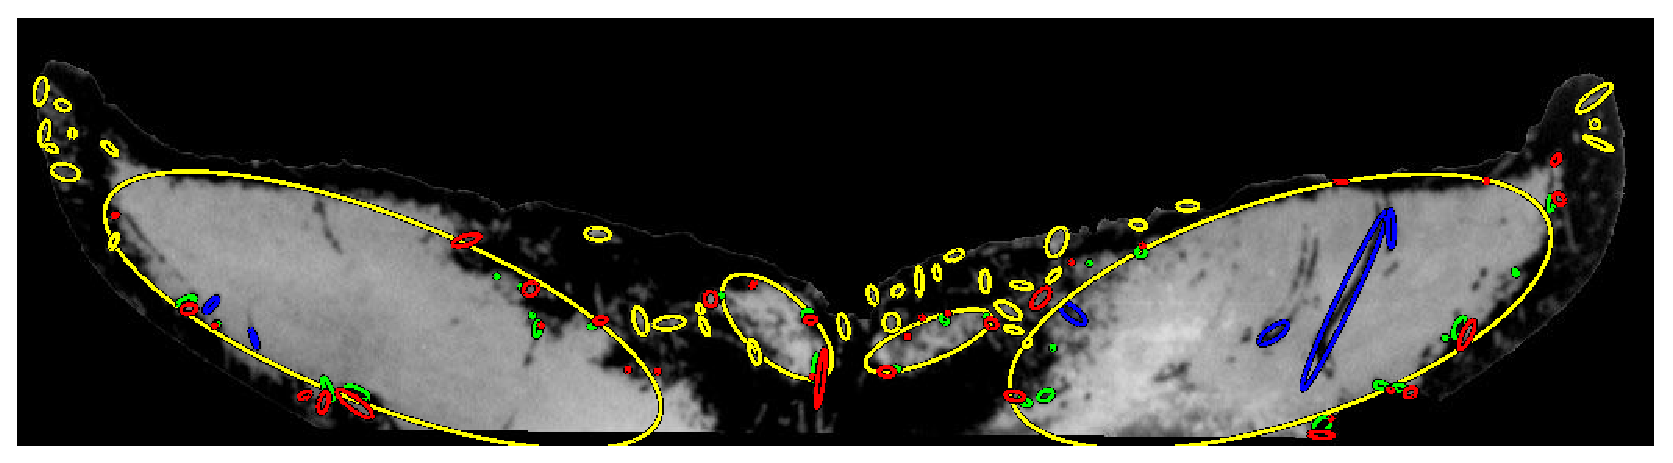
\includegraphics[width=4cm]{./Figs/dmsrTailB}}
\end{minipage}
\hfill
\vspace{-0.4cm}
\caption{Region detection on two images of the tail of the same humpback whale. 
Top row: MSER, bottom row: DMSR(All).}
\label{fig:tails}
\vspace{-0.3cm}
\end{figure}

%----------------------------------------------------------------
\begin{figure}[htb]

\begin{minipage}[b]{.24\linewidth}
  \centering
  \centerline{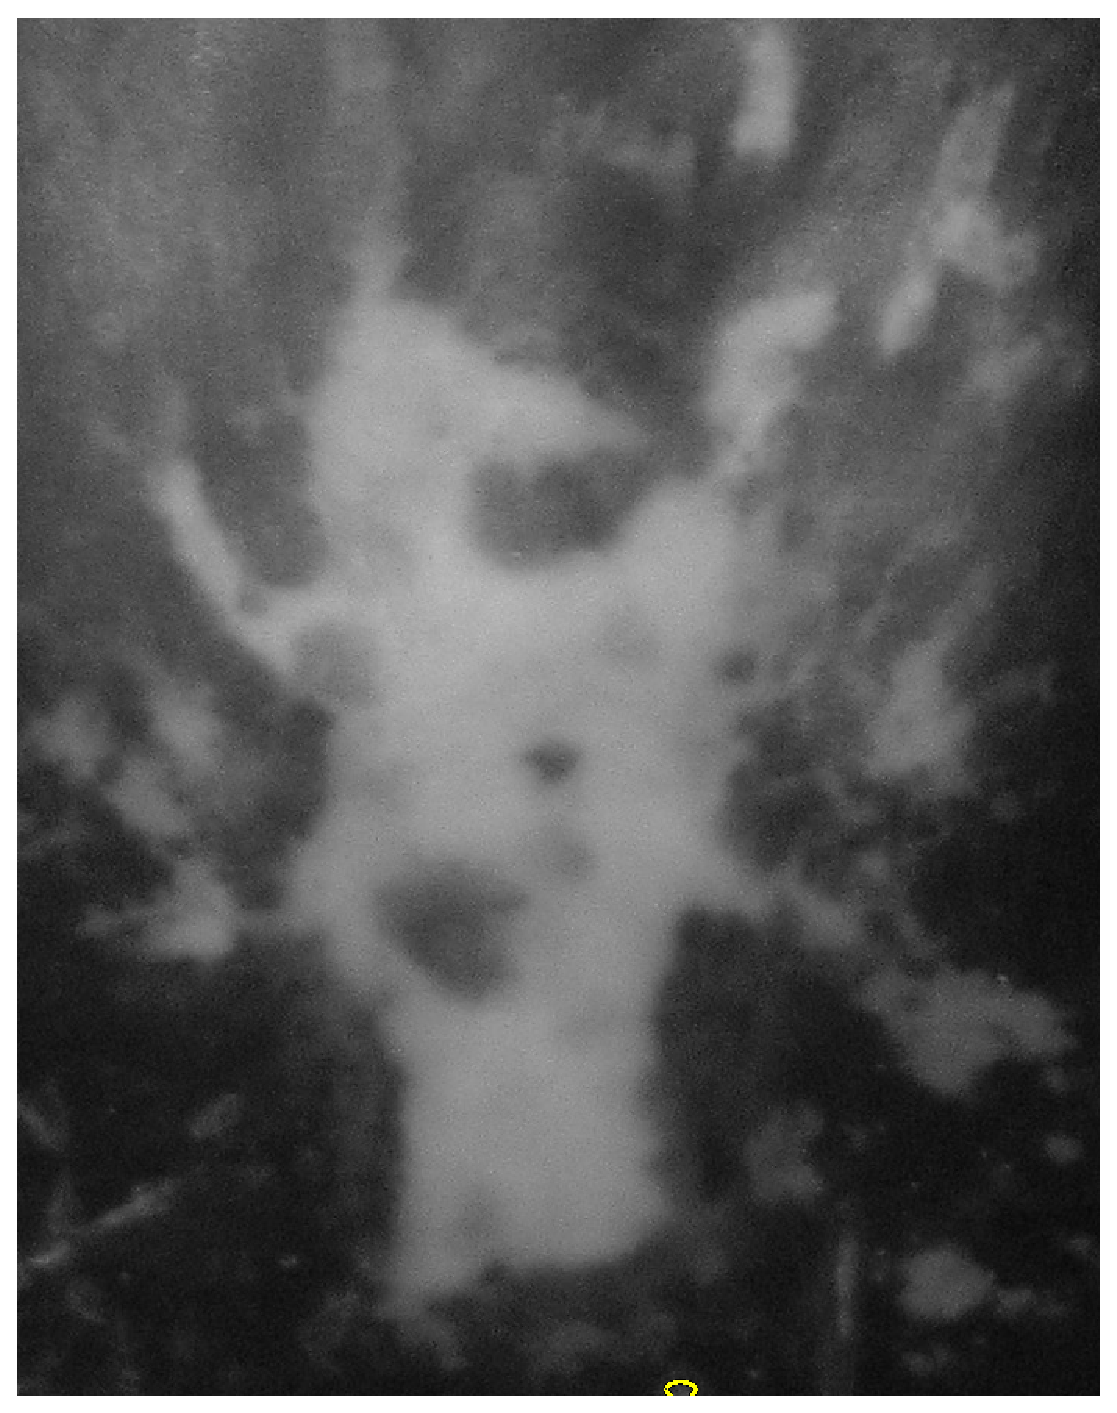
\includegraphics[width=1.8cm]{./Figs/mserLeatherbackA}}
   \centerline{(a)}\medskip
\end{minipage}
\hfill
\begin{minipage}[b]{0.24\linewidth}
  \centering
  \centerline{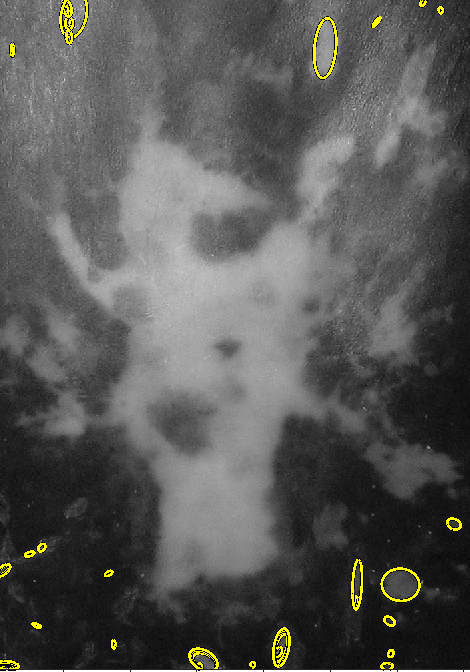
\includegraphics[width=1.8cm]{./Figs/mserLeatherbackB}}
\centerline{(b)}\medskip
\end{minipage}
\hfill
\begin{minipage}[b]{.24\linewidth}
  \centering
  \centerline{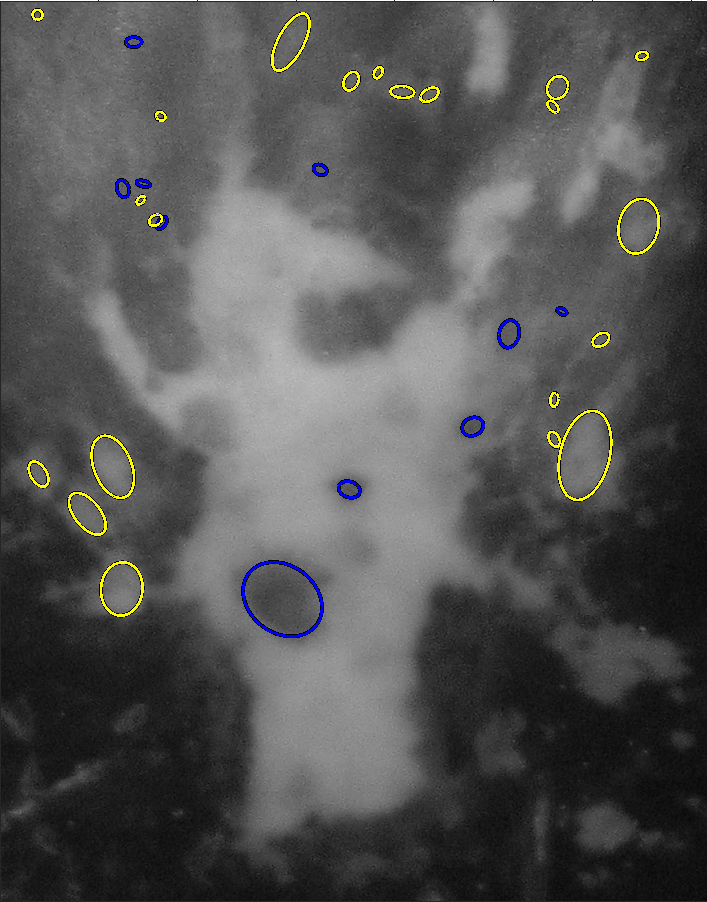
\includegraphics[width=1.8cm]{./Figs/dmsrLeatherbackA}}
\centerline{(c)}\medskip
\end{minipage}
\hfill
\begin{minipage}[b]{0.24\linewidth}
  \centering
  \centerline{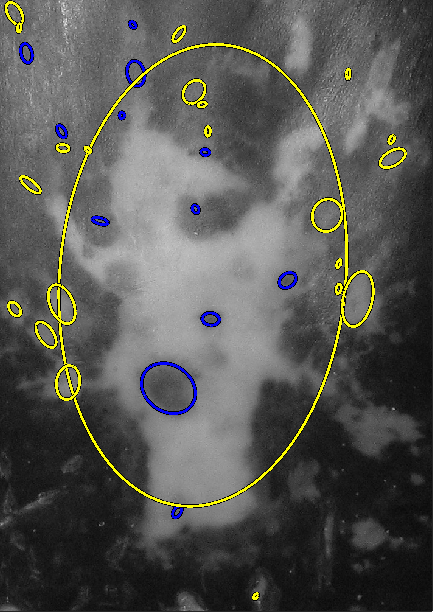
\includegraphics[width=1.8cm]{./Figs/dmsrLeatherbackB}}
 \centerline{(d)}\medskip
\end{minipage}
 \vspace{-0.2cm} 
\caption{Region detection on two images of the pineal spot of the same leatherback turtle.
(a),(b): MSER, (c),(d): DMSR.}
\label{fig:turtle}
 \vspace{-0.2cm}
\end{figure}

\end{comment}
Since then, many researchers have proposed improvements to MSER with no drastic increase of performance. An MSER color extension, {\em Maximally Stable Color Region}, outperforms both an MSER-per-color-channel combination and a color blob detector \cite{Forssen07}. Improving the MSER region distinctiveness by morphological dilation on the detected Canny edges is proposed in \cite{Wang14}. The improved detector shows better performance in classification application, but evaluation of repeatability is not reported. MSER has been extended to {\em Maximally Stable Volumes} for successful segmentation of 3D medical images and paper fiber networks \cite{DonoserB06}.

While most research has focused on generic applications, the emerging fields of {\em animal and plant biometrics} are attracting more attention \cite{Kuehl2013, leafsnap_eccv2012}. Computer vision is becoming a vital technology enabling the wild-life preservation efforts of ecologists in the big data era. Along with the individual or species photo-ID, the scientists wish to obtain reliable measurements of meaningful structures from images. The generic region detectors do not satisfy this need: Fig.\,\ref{fig:tails}, top row shows over-abundant or not semantic regions and Fig.\,\ref{fig:turtle}, (a), (b) shows missed detection. On the contrary, our {\em Data-driven Morphology Salient Regions (DMSR) detector} finds the semantic regions (Fig.\,\ref{fig:tails}, bottom row and Fig.\,\ref{fig:turtle}, (c), (d)). 


Although crucial for the development of detectors, there is a shortage of evaluation benchmarks, especially for performance analysis independently of the image content. The standard {\em Oxford dataset} is very small: eight test sequences containing six (one base and five transformed) images of the same scene each. Every pair (base, transformed) is related via a given transformation matrix (homography) \cite{Mikolajczyk:2005}.  The {\em Freiburg dataset} contains $416$ higher resolution images, generated by transforming $16$ base images in order to de-tangle transformations from content \cite{FischerDB14}.  
The {\em TNT dataset} contains versions of the same viewpoint sequences with increasing resolution from $1.5$ to $8$~MPixel per image. Highly accurate image pair homographies are given. It is suitable for evaluating robustness to resolution rather than to transformations \cite{CorRos2013}. 

This paper contributes to solving the identified problems. We propose a new regions detector, DMSR, and made the software available as open source \cite{elena_ranguelova_2016_45156}. It is related to the {\em Morphology-based Stable Salient Regions (MSSR)} detector that we developed in the context of humpback whale identification \cite{RangMSSR06, RangHumpb06}. DMRS includes a binarization, robust-to-lighting-and-blur, that yields a much smaller number of regions and is more stable across transformations. It has similar or higher (lighting, blur and increased resolution) repeatability compared to MSER, while detecting non-redundant perceptually salient regions (Fig.~\ref{fig:tails}). Also, we compose and share an openly available dataset, OxFrei, combining the natural homographies of the Oxford and the higher resolution images of the Freiburg datasets \cite{elena_ranguelova_2016_45156}.


\subsection{Subsection Heading Here}
Subsection text here.


\subsubsection{Subsubsection Heading Here}
Subsubsection text here.


% An example of a floating figure using the graphicx package.
% Note that \label must occur AFTER (or within) \caption.
% For figures, \caption should occur after the \includegraphics.
% Note that IEEEtran v1.7 and later has special internal code that
% is designed to preserve the operation of \label within \caption
% even when the captionsoff option is in effect. However, because
% of issues like this, it may be the safest practice to put all your
% \label just after \caption rather than within \caption{}.
%
% Reminder: the "draftcls" or "draftclsnofoot", not "draft", class
% option should be used if it is desired that the figures are to be
% displayed while in draft mode.
%
%\begin{figure}[!t]
%\centering
%\includegraphics[width=2.5in]{myfigure}
% where an .eps filename suffix will be assumed under latex, 
% and a .pdf suffix will be assumed for pdflatex; or what has been declared
% via \DeclareGraphicsExtensions.
%\caption{Simulation results for the network.}
%\label{fig_sim}
%\end{figure}

% Note that the IEEE typically puts floats only at the top, even when this
% results in a large percentage of a column being occupied by floats.


% An example of a double column floating figure using two subfigures.
% (The subfig.sty package must be loaded for this to work.)
% The subfigure \label commands are set within each subfloat command,
% and the \label for the overall figure must come after \caption.
% \hfil is used as a separator to get equal spacing.
% Watch out that the combined width of all the subfigures on a 
% line do not exceed the text width or a line break will occur.
%
%\begin{figure*}[!t]
%\centering
%\subfloat[Case I]{\includegraphics[width=2.5in]{box}%
%\label{fig_first_case}}
%\hfil
%\subfloat[Case II]{\includegraphics[width=2.5in]{box}%
%\label{fig_second_case}}
%\caption{Simulation results for the network.}
%\label{fig_sim}
%\end{figure*}
%
% Note that often IEEE papers with subfigures do not employ subfigure
% captions (using the optional argument to \subfloat[]), but instead will
% reference/describe all of them (a), (b), etc., within the main caption.
% Be aware that for subfig.sty to generate the (a), (b), etc., subfigure
% labels, the optional argument to \subfloat must be present. If a
% subcaption is not desired, just leave its contents blank,
% e.g., \subfloat[].


% An example of a floating table. Note that, for IEEE style tables, the
% \caption command should come BEFORE the table and, given that table
% captions serve much like titles, are usually capitalized except for words
% such as a, an, and, as, at, but, by, for, in, nor, of, on, or, the, to
% and up, which are usually not capitalized unless they are the first or
% last word of the caption. Table text will default to \footnotesize as
% the IEEE normally uses this smaller font for tables.
% The \label must come after \caption as always.
%
%\begin{table}[!t]
%% increase table row spacing, adjust to taste
%\renewcommand{\arraystretch}{1.3}
% if using array.sty, it might be a good idea to tweak the value of
% \extrarowheight as needed to properly center the text within the cells
%\caption{An Example of a Table}
%\label{table_example}
%\centering
%% Some packages, such as MDW tools, offer better commands for making tables
%% than the plain LaTeX2e tabular which is used here.
%\begin{tabular}{|c||c|}
%\hline
%One & Two\\
%\hline
%Three & Four\\
%\hline
%\end{tabular}
%\end{table}


% Note that the IEEE does not put floats in the very first column
% - or typically anywhere on the first page for that matter. Also,
% in-text middle ("here") positioning is typically not used, but it
% is allowed and encouraged for Computer Society conferences (but
% not Computer Society journals). Most IEEE journals/conferences use
% top floats exclusively. 
% Note that, LaTeX2e, unlike IEEE journals/conferences, places
% footnotes above bottom floats. This can be corrected via the
% \fnbelowfloat command of the stfloats package.




\section{Conclusion}
The conclusion goes here.




% conference papers do not normally have an appendix



% use section* for acknowledgment
\ifCLASSOPTIONcompsoc
  % The Computer Society usually uses the plural form
  \section*{Acknowledgments}
\else
  % regular IEEE prefers the singular form
  \section*{Acknowledgment}
\fi


The authors would like to thank...





% trigger a \newpage just before the given reference
% number - used to balance the columns on the last page
% adjust value as needed - may need to be readjusted if
% the document is modified later
%\IEEEtriggeratref{8}
% The "triggered" command can be changed if desired:
%\IEEEtriggercmd{\enlargethispage{-5in}}

% references section

% can use a bibliography generated by BibTeX as a .bbl file
% BibTeX documentation can be easily obtained at:
% http://mirror.ctan.org/biblio/bibtex/contrib/doc/
% The IEEEtran BibTeX style support page is at:
% http://www.michaelshell.org/tex/ieeetran/bibtex/
%\bibliographystyle{IEEEtran}
% argument is your BibTeX string definitions and bibliography database(s)
%\bibliography{IEEEabrv,../bib/paper}
%
% <OR> manually copy in the resultant .bbl file
% set second argument of \begin to the number of references
% (used to reserve space for the reference number labels box)

\bibliographystyle{IEEEtran}
\bibliography{aiccsa2016}


% that's all folks
\end{document}


